\chapter{Background and Related Work}
\label{c:related}
    \section{Representation}
    \label{s:related:representation}
    A 3D object can be represented with different models.
    The most popular representation of 3D objects is polygonal meshes, 
    especially the triangle meshes.
    %, because most graphic cards are optimized for triangle meshes. 
    Point-based representations are also used in practice.
    A point-based representation can be considered as a 
    sampling of a continuous surface, resulting in a set of 3D points. 
    To bridge the gaps between neighboring point samples, 
    bounding spheres \cite{rusinkiewicz:qsplat, 364350} or surface splats \cite{383300} are used as rendering primitives. 
    More details about point-based models can be seen in the survey by Kobbelt and Botsch \cite{DBLP:journals/cg/KobbeltB04} 
    and the PhD thesis of Wand \cite{wand:point}.  
    In addition to these surface modeling methods, 
    constructive solid geometry (CSG), a commonly used technique used in solid modeling, 
    constructs visually complex 3D objects with applying boolean operations
    (such as union, intersection, and difference) on simple solid objects,
    such as cubes, spheres, cylinders, cones, and  pyramids. 
    CSG is extensively used in game development and CAD applications, because it is 
    relatively easy to be constructed manually with computers and provides mathematical accuracy. 
    As a specific example, we have used generalized cylinders to represent and streaming plants 
    \cite{plant:seb, compact:mondet}.

    This thesis concentrates on meshes because of following reasons:
    \begin{itemize}
        \item Most rendering hardware are optimized for meshes, so other model needs to be convert
            to meshes before rendering either explicitly or implicitly. 
        \item Without connectivity information in the model, point-based model is relatively easier to deal with
            than meshes. Therefore, adapting techniques used in streaming meshes to streaming point-based model
            is easier than the opposite direction.
    \end{itemize}
    
    A triangle mesh can be donated as a tuple $(K, V)$, where $K$ is a
    \emph{simplicial complex} including all the mesh simplices 
    (vertices, edges and triangles) and $V =\{v_{1}, v_{2}, ...,
    v_{n}\}$ is the set of geometry positions of vertices. Therefore,
    a mesh has both \emph{connectivity} information represented by $K$
    and \emph{geometry information} represented by $V$. In other
    words, $K$ includes all the topology information of all the
    elements in the mesh. If
    polygons are allowed in $K$ instead of only triangles, then this
    kind of meshes are called polygonal meshes.

    In a mesh, it is required that every
    vertex is an end of an edge and every edge should be incident to at
    least one face (Figure \ref{mesh_non_mesh}(a) is not a mesh).
    The number of edges incident to a vertex is called the
    \emph{valence} of this vertex, and the number of edges incident to
    a face is called the \emph{degree} of this face. An edge that is 
    incident only to one face is called a \emph{boundary edge}; an edge
    shared by two faces is called an \emph{interior edge}; an edge
    shared by more than two faces is called a \emph{singular edge}. A
    \emph{manifold mesh} is a mesh without singular edges and every
    two faces share one edge or nothing (see Figure \ref{mesh_non_mesh}).
\begin{figure}
\centering
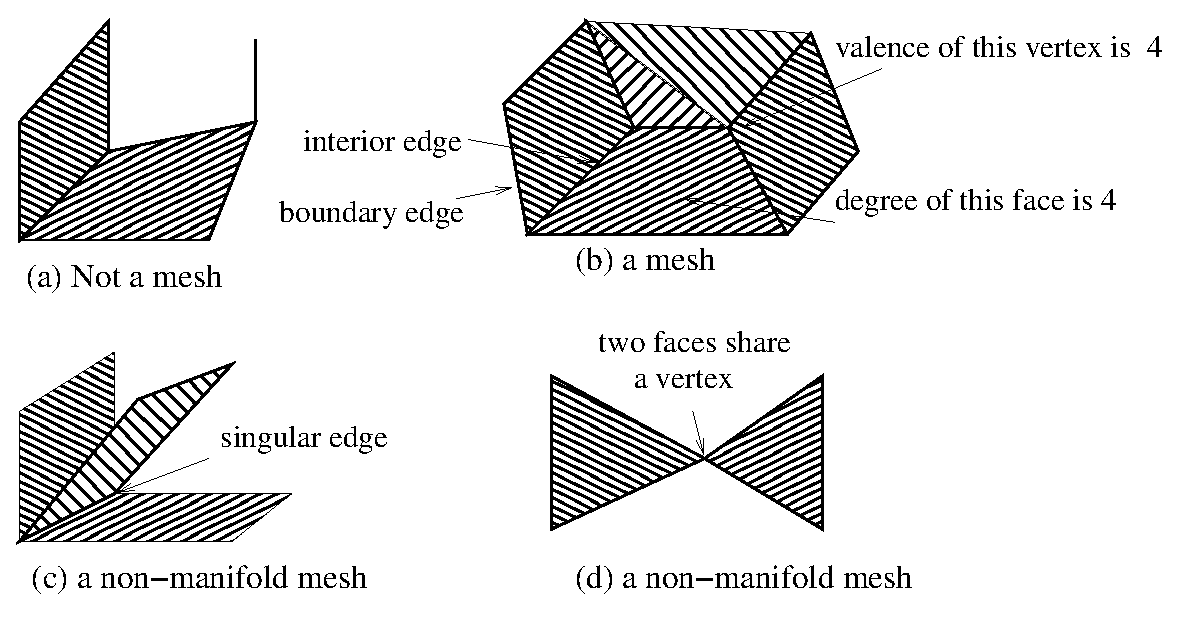
\includegraphics[width=0.8\textwidth]{figure2.1.eps}
\caption[Manifold mesh, non-manifold mesh and non-mesh]{ (a) is not
a mesh since one edge is incident to no face. (b) is a manifold
mesh. (c) is a non-manifold mesh since there is a singular edge.
(d) is a non-manifold mesh since two faces share only a
vertex.\label{mesh_non_mesh}}\
\end{figure}

    Polygonal meshes can be used as an approximation of the surfaces
    of 3D objects. In this case, some properties of the surface such
    as color and normal are often associated with the mesh. These
    properties can be categorized into two types: discrete attributes
    and scalar attributes\label{property}. Discrete attributes, such
    as material identifier, are usually associated with the faces, while
    scalar attributes, such as color, normal, and texture coordinate,
    are often associated with vertices or corners (the tuple (vertex,
    face)). The latter one is used because in the case of
    discontinuity, a vertex can have more than one scalar value. For
    example, if two smooth surfaces intersect at a curve, then vertices
    in this curve will have two different normal values. Therefore,
    the normal value should be associated with the tuple (vertex face).
    Then, polygonal meshes can be represented by $(K, V, D, S)$ where
    $D$ is the set of discrete attributes associated with face $f \in
    K$ and $S$ is the set of scalar attributes associated with corners $(v, f)$ in $S$.

    \section{Coding and Compression}
    A mesh is encoded first before it can be stored or
    transmitted. Coding represents a mesh with a sequence of
    bits. Compression is always combined with coding to save the storage space
    or the bandwidth needed in transmission. 
    There are two kinds of coding:
    single-rate coding and progressive coding. 
    Single-rate coded mesh can only be decoded when all data becomes available 
    whereas progressive coded mesh can be decoded with only part of the data is available. 
    We will briefly introduce single-rate coding methods, and then concentrate on
    progressive coding methods, because the latter are more suitable for progressive streaming.
    
    \subsection{Single-rate Coding} \label{single_rate}
    In a mesh, three kind of information needs to be coded:
    connectivity, geometry and property. 
    Since most property data are associated with vertices, 
    many compression algorithms either treats them as geometry data or 
    ignore them. We first introduce connectivity coding, 
    and then introduce geometry coding briefly.
    
    A triangle mesh is often represented as an array of vertex coordinates
    (geometry information) and an array of triangles (connectivity information). 
    A triangle is represented by the indices of its three vertices,
    where every vertex is indexed by all the
    triangles to which it is incident. Repeated references to the triangles introduce
    redundancy. Such redundancy can be reduced using either 
    %Therefore, triangle strip method is introduced to
    %reduce this redundancy. In a 
    triangle strip, a triangle fan, or a
    generalized triangle strip (a mixture of triangle strips and
    triangle fans) (see Figure \ref{strip}), 
    in which triangles are represented with one index of vertex
    except the first triangle. 
    Deering \cite{218391} first introduced generalized triangular mesh, 
    which combining the generalized triangle strips with a vertex buffer
    to further reduce the bits used to represent indices. 
    Furthermore, Chow \cite{267103} introduced a method to
    decompose a mesh into triangle strips. 
    Bajaj, Pascucci and Zhuang \cite{789628} presented a coding method with layered
    decomposition. 
    Typically, a triangle layer is a generalized triangle strip. 
    \begin{figure}[ht]
    \centering
    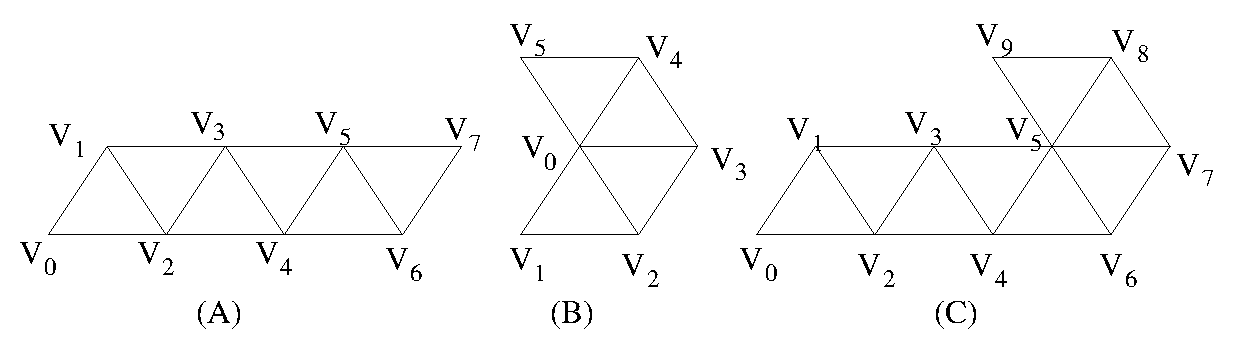
\includegraphics[width=0.6\textwidth]{strip.eps}
    \caption{(a) The triangle strip, (b) the triangle fan, and (c) the generated triangle strip.}\label{strip}
    \end{figure}

    Taubin and Rossignac \cite{274365} proposed a method named
    \emph{topological surgery}, which changes coding of a manifold
    mesh to coding of two trees: a vertex spanning tree and the dual of the triangles.
    Topological surgery has been implemented in MPEG-4 standard, and more details
    can be seen in the report of Taubin \cite{3d:Taubin}.
    
    Touma and Gotsman \cite{triangle:Touma} introduced a
    valence-driven approach to encode the connectivity by coding the
    valence of all the vertices in a specific traversing order. 
    The performance is further improved
    by Alliez and Desbrun \cite{alliez01valencedriven}, who also proved a
    upper-bound 3.24 bpv, exactly the theoretical value computed
    by Tutte \cite{census:Tutte} after enumerating all possible planar
    graphs.

    Gumhold and Stra\ss{}er proposed a method called \emph{cut-border machine} \cite{280836}.
    A significant advantage of this method is that it can be easily implemented
    in hardware and the decompression is fast, which
    makes it very useful for real-time coding. 
    Another method named \emph{edgebreaker} is presented by Rossignac \cite{614421}.
    It is similar to the cut-border machine but has better
    compress efficiency and much slower decompression speed.
    
    After introduction of connectivity coding, we briefly introduce geometry
    coding. Most single-rate geometry compression methods involve three steps:
    quantization, prediction, and entropy coding.

    In VRML, geometry data is represented with 32 bit floating-point
    number, but this precision is highly beyond the perceiving
    capability of human eyes. Hence, quantization can be performed to
    compress the geometry data. Typically, each coordinate in a mesh is
    uniformly quantized to 8-16 bits integer.

    After quantization of vertex coordinates, prediction is taken in
    encoding by exploiting correlations between adjacent vertex
    coordinates. An effective prediction scheme generates prediction
    errors with highly compact distribution, which can be effectively
    encoded by entropy coders, such as Huffman coder or arithmetic
    coder. 

    More details about single-rate coding can be seen in the tutorial
    by Gotsman, Gumhold, and Kobbelt \cite{gotsman-simplification},
    the survey by Taubin \cite{3d:Taubin}, by Alliez and Gotsman
    \cite{recent:alliez}, and the survey by Peng, Kim and Kuo
    \cite{technologies:peng}.
    
    \subsection{Progressive Coding}
    %(TODO add survey of geometric images)
    Single-rate coded meshes can only be decoded after they are
    completely received, so they are not suitable for streaming. Therefore,
    some progressive coding schemes have been proposed. According to
    how the original mesh is simplified, these coding scheme can be
    categorized into three classes: progressive mesh-based, vertex
    clustering-based, and re-meshing-based.
    
    \begin{description}
        \item[Vertex Clustering-Based] 
            In vertex clustering based schemes, space is divided into cells
            following regular structure such as kd-tree \cite{566591} and 
            octree \cite{1073237}. All vertices inside a cell are represented
            by one delegate. Cells can be further divided into smaller cells
            and the quality of reconstructed model increases. Vertex clustering
            based coding can code geometry information efficiently, but it is 
            difficult to code connectivity information. Moreover, the quality
            of base mesh is poor.

        \item[Re-meshing-Based]
            Re-meshing based method only keeps the shape of a model
            and does not keep the accurate topology. 
            An irregular mesh can be converted into a semi-regular mesh
            with similar shape. 
            %In a semi-regular
            %triangle mesh, the valence of most vertices is six, and therefore
            Because of the regularity of the new mesh,
            the connectivity information can be coded almost without cost.
            %More details about these algorithms can be seen in the survey by Allienz and Gotsman
            %\cite{recent:alliez}, the survey by Peng, Kim and Kuo
            %\cite{technologies:peng} and the references therein.
            In 2002, Gu et al. proposed an algorithm to remesh a
            mesh to a completely regular structure and represented it 
            as a \emph{geometry image} \cite{gu:geometry}. 
            Geometry, color, and normal information
            of a 3D mesh then can be stored all as 2D images. Therefore,
            traditional image processing techinique can be used.
            For example, spectral geometry processing are studied by many researchers
            \cite{taubin:signal, karni:spectral}
            and a state-of-art survey was done by Zhang et al. \cite{zhang:spectral}.
            He et al. proposed \emph{spectral geometry images} to generate more 
            visually pleasing shape with higher compression efficiency. Moreover, 
            they proposed an error protection scheme to target networks with 
            packet loss \cite{he:spectral}.
            %Besides losing the correct topology information,
            %re-meshing based methods usually code a mesh as a whole, 
            %so there is no flexibility in streaming order.

        \item[Progressive Mesh-Based]
            In this thesis, we concentrate on progressive meshes, which provide 
            the finest granularity in choosing streaming order and subset, 
            so we introduce the progressive mesh based coding in more details.
    \end{description}

    The progressive mesh (PM) \label{progressive_mesh}is first
    introduced by Hoppe in 1996 \cite{hoppe96progressive}. In this
    scheme, the simplification is based on \emph{edge collapse}, which
    collapses an edge into a vertex (see Figure \ref{split2}).
    After a series of edge collapse, a coarser \emph{base mesh} remains. 
    Then the PM is constructed by the base mesh and a series of \emph{vertex
    splits}, the inverse of edge collapse, in a reverse order.
    Different level-of-detail can be achieved by applying different number
    of vertex splits.
    %Rendering can be done  n receiver side at any time after the base
    %mesh is received. More vertex splits received, better
    %approximation to the original mesh generated. After all
    %the vertex split operations are received, the original mesh can be
    %reconstructed without loss\footnote{quantization error may exist
    %when quantization is taken in geometry compression.}.

    The base mesh can be encoded with the single-rate coding methods
    introduced in section \ref{single_rate}. Here, we introduce
    how to encode the vertex splits. 
\begin{figure}
\centering
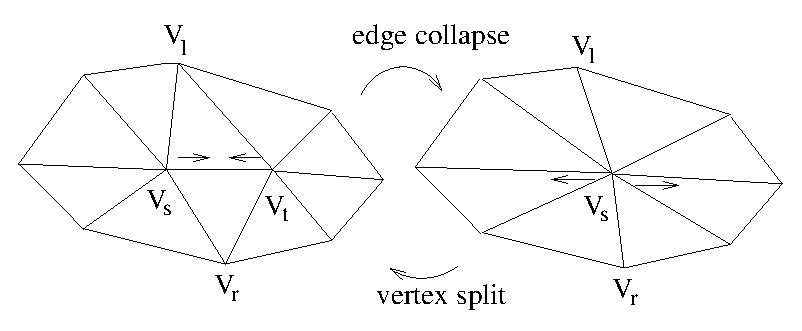
\includegraphics[width=0.5\textwidth]{split2.eps}
\caption{Edge collapse and vertex split}\label{split2}
\end{figure}
    For connectivity
    information, we need to code $s$, $l$, and $r$, and for geometry
    information, we need to code the new position of $v_{s}$ and the
    position of $v_{r}$. If half collapse, which always collapse an
    edge to one of its ends (i.e. $v_{s}$ keeps unchanged), is used, 
    we only need to code the position of $v_r$. 
    
    If the number of vertices in current model is
    $V$, then $s$ can be any one of them, 
    and ${\lceil}log_{2}V{\rceil}$ bits are needed to encode $s$. 
    
    Many compression methods are proposed to reduce this cost.
    Hoppe \cite{efficient:hoppe} present an efficient implementation,
    in which the vertex splits are ordered such that next one
    is as close to current one as possible. This method reduces the cost
    from $O(Vlog_{2}V)$ to $O(V)$.
    Karni, Bogomjakov, and Gotsman \cite{602153}, 
    also use specific order of vertex split to reduce the cost of connectivity. 
    The vertex sequence is generated by recursively cutting a mesh into two
    balanced part with minimum cut. With their algorithm, the connectivity can
    be encoded with in average 4.5 bpv. 

    Another idea is to group many vertex splits together, 
    and efficiency can be improved at the cost of coarser granularity. 
    Taubin, Gu\'{e}ziec, Horn, and Lazarus \cite{280834} proposed the
    progressive forest split scheme (PFS), in which several edge
    collapse operations are combined together and the inverse operation splits a
    forest of edges and vertices. 
    Payarola and Rossignac \cite{614450}, 
    proposed compressed progressive mesh (CPM)\label{cpm} with similar
    idea. They group about $50\%$ vertex splits into one batch. To
    differentiate vertices to be split with others, one bit per vertex
    is used as indicative. 
    Other methods have the similar idea
    but based on vertex removal (remove a vertex and triangulates the hole
    generated) \cite{319358}. 

    More methods exist to reduce the cost in encoding connectivity information.
    Some of them are extended from the single rate coding algorithms
    \cite{319426, 383281}. Some extend progressive mesh to directly
    encode non-manifold meshes \cite{258852}.

    All compression methods introduced above 
    have a common drawbacks. After compression, the 
    data becomes linear and has to be decoded in a fix order. 
    Therefore, these methods improve the coding efficiency at the cost
    of losing flexibility, which is essential in streaming of high-resolution
    progressive meshes.
    
    Flexibility of choosing streaming order 
    is restricted by the dependency among the vertex splits.
    For a manifold mesh, a vertex split operation depends on the existence of
    \begin{itemize}
        \item 
    the vertex to be split ($V_s$ in Figure \ref{split2}), 
        \item 
    two cut neighbors ($V_l, V_r$ in Figure \ref{split2}). 
    \end{itemize}
    More dependencies exist if artificial folds are strictly forbidden \cite{258843, 258847}, 
    but in this thesis we ignore these dependencies since we can 
    tolerate temporary folds in our scheme.
     
    To et al. \cite{To1999} further removed the second dependency.
    In their method, if a cut neighbor does not exist during a vertex split,
    its ancestor are used as the cut neighbor instead.
    Kim and Lee \cite{kim01truly} improved this method so that the final mesh
    can keep the original connectivity. 
    Kim et al. \cite{multiresolution:kim} proposed a better scheme that enables
    an ordinary progressive mesh to be split in random order.

    These methods increase the flexibility, but reduce coding efficiency.
    One solution proposed by Yang et al. \cite{progressive:Yang}
    is to divide the whole mesh into several segments and encode them
    separately to trade off between flexibility and compression efficiency.
    The weakness is that the size of the base mesh is relatively large
    since the original vertices in the border of segments are kept in the base
    mesh. Furthermore, the quality of the base mesh is uneven.

    Kim et al. \cite{multiresolution:kim}
    have proposed a compression algorithm that allows random splitting of a mesh without
    sacrificing compression efficiency. This method is neat since it achieves comparable
    efficiency with other compression methods but maintains the highest flexibility.
    This algorithm, however, is not designed for 
	network transmission.  We extend this algorithm in this thesis. More details are introduced
    in Chapter \ref{c:rdstream}.  
    
    \section{3D streaming}
    \label{s:related:streaming}
    Given the backgrounds in modeling and coding, now we introduce some
    related works in 3D streaming. 
    The main concern in 3D streaming is how to improve the quality of the received
    mesh as fast as possible. Current studies can be categorized into three groups
    by how to achieve this objective.
    %Three main classes of work exist 
    %-- error resilient streaming, packetization, and view-dependent streaming.
    
    \subsection{Error Resilient Streaming}
    To improve the quality quickly, we need to mitigate distortion of the 
    rendered quality of rendered mesh in the presence of packet losses.

    At the transport layer, Al-Regib and Altunbasak \cite{3tpregib}, Li
    et al. \cite{Li2006, li:3dmulticast}, and Chen et al. \cite{chen05hybrid} have
    investigated how to intelligently select either TCP or UDP for
    transmissions to trade off reliability and end-to-end delay.  Li et
    al. have also considered SCTP with partial reliability.
    Harris III and Kravets \cite{harris:design} proposed a new
    transport protocol that exploits loss tolerance and
    partially-ordered property of 3D objects organized into trees of
    bounding volumes.

    At the application layer, the major error control techniques: error
    resilient coding, error protection, retransmission, and error
    concealment \cite{Park2003}, have all been applied to mesh streaming.  
    
    Existing work in robust mesh compression aims to
    reduce dependencies among the mesh \cite{error:Park,error:Yan}.
    Similar to introducing key frames or restart marker in video/image
    coding, mesh segmentation is used to reduce the affected range of one
    packet loss. In robust mesh compression, a mesh is typically
    partitioned into several independent segments and then coded separately.
    Therefore the effect of one packet loss is confined to the segment to which
    it belongs. The finer the partition is, the fewer the affected vertices
    are.  The coding efficiency, however, decreases
    due to more redundancies and less correlation.

    Al-Regib and Altunbasak \cite{unequal:Al-Regib} proposed an
    unequal error protection method to improve the resilience of
    progressive 3D mesh based on CPM (compressed progressive meshes). 
    Forward error correction (FEC) codes are added to the
    base mesh and additional levels-of-detail information to maximize 
    the decoded mesh quality.  The method is similar to FEC protection 
    of video data.

    Chen et al. \cite{chen05hybrid} also applied FEC to streaming
    progressive meshes. They analyzed several transmission schemes:
    TCP only, UDP only, TCP with UDP, and UDP with FEC, and studied
    their effects experimentally on the transmission time and decoded
    mesh quality.

    Cheng et al. \cite{loss:cheng} proposed a sending strategy of mesh
    with textures based on sub-sampling. 
    Their objective is to optimize the perceptional quality, which depends 
    on both geometry quality and texture quality. 
    
    Some studies use retransmission to recover the packet loss.
    For example, Tian \cite{Tian2006} uses selective retransmission in their system.
    We think that retransmission is more suitable than FEC when the feedback
    channel is available, because there is no playback deadline in streaming
    of 3D meshes and data is always useful.

    Most of methods introduced above treat the meshes streamed as 
    traditional linear data. When the flexibility of progressive mesh
    is considered, a new question arises: how to select a sending order
    to improve the quality quickly and mitigate the effect of packet loss.
    We call it the \emph{packetization} problem.
    
    \subsection{Packetization}
    \label{ss:intro:packetization}
    Packetization is tackled by
    Harris III and Karvets in \cite{harris:design}.   
    They proposed a protocol named On-Demand Graphic Transport Protocol (OGP)
    for transmitting 3D models represented as a tree of bounding volumes.
    A key component of the protocol is to decide which bounding volumes
    to send.  OGP begins with packing the largest possible subtree at
    the root and continues to pack the nodes in the subtree of
    acknowledged nodes in breadth-first order.  
    
    Gu and Ooi \cite{Gu:Packetization} were the first to look at
    the packetization problem for progressive meshes.  They model
    the packetization problem as a graph problem where the objective
    is to equally partition the graph into $k$ partitions with minimum
    cut size.  The problem is shown to be NP-complete and a heuristic
    is proposed.  They, however, assume that every vertex split contributes 
    equally to the rendered quality.
    
    In practice, the contribution of vertex splits can
    vary considerably. Therefore, when choosing sending order, we
    need to trade off between minimizing the dependency and sending 
    vertex split with higher contribution first. To achieve this objective,
    the effect of dependency needs to be quantitatively measured.
    There is no existing study is done for this problem
    prior to this thesis.

    A commonly used metric of contribution of vertex splits is 
    Hausdorff distance between the original and reconstructed mesh \cite{cignoni98metro}.
    As Hausdorff distance is view independent, 
    bandwidth may be wasted in sending invisible vertex splits
    before the visible ones. Moreover, even among the visible vertex splits,
    the view-independent metric cannot reflect the real contribution to the visual quality of
    clients with different viewpoints. A vertex split that significantly
    changes a mesh may change the rendered image 
    only slightly.  A better metric for visual contribution of a vertex split,
    based on the rendered image on the screen, 
    needs to consider the receiver's viewpoint.
    Streaming of 3D models based on this metric is named \emph{view-dependent} streaming.

    \subsection{View-Dependent Streaming}
    The view-dependent approach first appeared as 
    a dynamic simplification method used for adaptive rendering of a complex 3D mesh
    \cite{258843, 258847}. Only vertex splits that contribute to the rendered
    image will be rendered, allowing real-time rendering of a complex mesh
    even with limited rendering capability.
    Besides progressive mesh, other multi-resolution representations, 
    such as vertex-clustering  and subdivision scheme,
    are used in view-dependent refinement systems \cite{245627, efficient:Alliez,602344}.

    Later, the view-dependent approach is used in progressive 
	streaming of 3D meshes.     
    In the scheme proposed by Southern et al. \cite{363375},  the client is stateless and
    maintains only the visible data. 
    To et al. \cite{To1999}
    and Kim et al. \cite{kim:view} proposed that received data are stored
    in the receiver even after they become invisible, 
    so they need not be resent when they are visible again. 
    In these papers, view-dependent approaches mainly aim at addressing
    limited rendering capability. 
    
    Yang et al. \cite{progressive:Yang} and
    Zheng et al. \cite{zheng:interactive}, on the other hand, use
    view-dependent streaming to address limited network bandwidth.
    Yang et al. proposed a scheme where the server chooses the appropriate resolution
    according to the available network bandwidth.
    Zheng et al. \cite{zheng:interactive} use prediction to
    reduce the effect of network latency and 
    compensate the round-trip delay with the rendering time.
    Moreover, Yang et al. \cite{optimized:yang} proposed an joined 
    optimizing transmission method based on a general rate-distortion
    model that considers both mesh and texture data. Their method
    allocates bits between mesh and texture to optimize the display 
    quality at every stage of progressive transmission.
     
    These systems use sender-driven approach and do not address
    server scalability issues. Due to the stateful design, 
    the sender-driven approach is difficult to be extended to
    support caching proxy and peer-to-peer techniques, two 
    common solutions to scalability. This thesis presents the first
    scalable 
    view-dependent streaming system without incurring high infrastructural cost.
    

